%%%%%%%%%%%%%%%%%%%%%%%%%%%%%%%%%%%%%%%%%
% Short Sectioned Assignment LaTeX Template Version 1.0 (5/5/12)
% This template has been downloaded from: http://www.LaTeXTemplates.com
% Original author:  Frits Wenneker (http://www.howtotex.com)
% License: CC BY-NC-SA 3.0 (http://creativecommons.org/licenses/by-nc-sa/3.0/)
%%%%%%%%%%%%%%%%%%%%%%%%%%%%%%%%%%%%%%%%%

%----------------------------------------------------------------------------------------
%	PACKAGES AND OTHER DOCUMENT CONFIGURATIONS
%----------------------------------------------------------------------------------------

\documentclass[paper=a4, fontsize=11pt]{scrartcl} % A4 paper and 11pt font size

% ---- Entrada y salida de texto -----

\usepackage[T1]{fontenc} % Use 8-bit encoding that has 256 glyphs
\usepackage[utf8]{inputenc}

% ---- Idioma --------

\usepackage[spanish, es-tabla]{babel} % Selecciona el español para palabras introducidas automáticamente, p.ej. "septiembre" en la fecha y especifica que se use la palabra Tabla en vez de Cuadro

% ---- Otros paquetes ----

% Hipervínculos
\usepackage[hidelinks]{hyperref}

\usepackage{amsmath,amsfonts,amsthm} % Math packages
\usepackage{graphics,graphicx, float, url} %para incluir imágenes y colocarlas
% \usepackage{ulem}

\usepackage{fancyhdr} % Custom headers and footers
\pagestyle{fancyplain} % Makes all pages in the document conform to the custom headers and footers
\fancyhead{} % No page header - if you want one, create it in the same way as the footers below
\fancyfoot[L]{} % Empty left footer
\fancyfoot[C]{} % Empty center footer
\fancyfoot[R]{\thepage} % Page numbering for right footer
\renewcommand{\headrulewidth}{0pt} % Remove header underlines
\renewcommand{\footrulewidth}{0pt} % Remove footer underlines
\setlength{\headheight}{13.6pt} % Customize the height of the header

\numberwithin{equation}{section} % Number equations within sections (i.e. 1.1, 1.2, 2.1, 2.2 instead of 1, 2, 3, 4)
\numberwithin{figure}{section} % Number figures within sections (i.e. 1.1, 1.2, 2.1, 2.2 instead of 1, 2, 3, 4)
\numberwithin{table}{section} % Number tables within sections (i.e. 1.1, 1.2, 2.1, 2.2 instead of 1, 2, 3, 4)

\setlength\parindent{0pt} % Removes all indentation from paragraphs - comment this line for an assignment with lots of text

\newcommand{\horrule}[1]{\rule{\linewidth}{#1}} % Create horizontal rule command with 1 argument of height

%% Para incluir archivos en texto plano
\usepackage{listings}

%----------------------------------------------------------------------------------------
%	TÍTULO Y DATOS DEL ALUMNO
%----------------------------------------------------------------------------------------

\title{	
\normalfont \normalsize 
\textsc{{\bf Ingeniería de Servidores (2015-2016)} \\ Doble Grado en Ingeniería Informática y Matemáticas \\ Universidad de Granada} \\ [25pt] % Your university, school and/or department name(s)
\horrule{0.5pt} \\[0.4cm] % Thin top horizontal rule
\huge Memoria Práctica 3 \\ % The assignment title
\horrule{2pt} \\[0.5cm] % Thick bottom horizontal rule
}

\author{Óscar Bermúdez Garrido\\ \href{http://www.github.com/oxcar103}{@oxcar103}} % Nombre y apellidos

\date{\normalsize\today} % Incluye la fecha actual

%----------------------------------------------------------------------------------------
% DOCUMENTO
%----------------------------------------------------------------------------------------

\begin{document}
\maketitle % Muestra el Título
\newpage %inserta un salto de página
\tableofcontents % para generar el índice de contenidos
\listoffigures

\begin{enumerate}
	\section{Monitorización de Sistemas Linux}
	\subsection{Conociendo el subsistema de archivos}
		\item 
		\begin{enumerate}
			\item ¿Qué archivo le permite ver qué programas se han instalado con el gestor de paquetes?
			
			La ubicación de estos archivos depende, como es lógico, del gestor de paquetes. Basándome
			en la sección de ficheros de los respectivos manuales de dichos gestores(\textit{apt}
			\cite{man_apt-get} en Ubuntu y \textit{yum}\cite{man_yum} en CentOS), los registros de los
			paquetes instalados serían:
			\begin{itemize}
				\item \verb|/var/cache/apt/archives| para \textit{apt-get}
				\item \verb|/var/cache/yum| para \textit{yum}.
			\end{itemize}
			
			Inspeccionando el directorio \verb|/var/log|, también descubrí otros ficheros que guardan
			registros sobre los paquetes instalados:
			\begin{itemize}
				\item En \textit{apt} se usa \verb|/var/log/apt/history.log| para los paquetes y
				\verb|/var/log/apt/terms.log| para los comandos de configuración.
				\item En \textit{yum}, todo  se almacena en \verb|/var/log/yum.log|
			\end{itemize}
			
			\item ¿Qué significan las terminaciones .1.gz o .2.gz de los archivos en ese directorio?
			
			En el directorio \verb|/var/log| se almacenan archivos con datos del sistema y de algunos
			programas y servicios. Por ejemplo, los datos de comienzo y cierre de sesión.\cite{dir_var}
			
			Para automatizar el proceso de creación y borrado de estos archivos, se hace uso de
			\textit{logrotate}\cite{man_logrotate} ejecutándose diariamente con \textit{cron}. Este
			comando, revisa los archivos log y, en función del archivo de configuración del servicio
			asociado, lo borra(si excede el tiempo establecido\footnote{Puede ser que lo que determine
			si un archivo de log debe ser borrado sea que hay muchas copias de log del servicio
			asociado, en cuyo caso, se borra la más antigua.}) o crea uno nuevo(si el actual tiene más
			tiempo del que está establecido\footnote{Puede ser que la condición para determinar si un
			archivo de log debe dejar de escribirse en él y empezar a escribir en otro nuevo sea que
			ha excedido cierto tamaño.}).
			
			Cada vez que se crea un nuevo archivo con \textit{logrotate}, su formato por defecto
			es $<$service\_name$>$.$<$other\_values$>$.$<$version\_number$>$.gz\footnote{Cada vez que
			se llama a \textit{logrotate}, se renombran los archivos, esto es, el más antiguo, será el
			que mayor número de versión tenga. Además, el primer archivo, no tendrá el número de
			versión.}, aunque este formato puede ser modificado en el correspondiente archivo de
			configuración.
		\end{enumerate}
		
	\subsubsection{Volviendo con el RAID1}
		\item \textbf{Opcional:} Indique qué comandos ha utilizado para realizarlo así como capturas
		de pantalla del proceso de reconstrucción del RAID.
		
		Para el fallo, usaremos el comando \verb|mdadm -–manage /dev/md0 –-fail /dev/sda1|
		\cite{man_mdadm} para marcar el dispositivo como defectuoso:
		
		\begin{figure}[H]
			\centering
			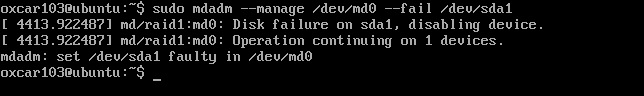
\includegraphics[width=15cm]{Ejercicio_2a.jpg}
			\caption{Marcamos el fallo del dispositivo.}
			\label{fig:mark}	
		\end{figure}
		
		Comprobamos con el monitor sugerido \verb|watch -c2 cat /proc/mdstat| que se ha logrado marcar
		con éxito, podemos ver una $"$F$"$ que(gracias a \cite{wiki_mdstat}) sabemos que significa que
		ese dispositivo está marcado con un fallo:
		
		\begin{figure}[H]
			\centering
			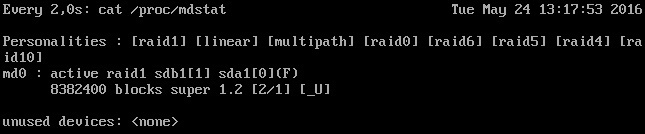
\includegraphics[width=15cm]{Ejercicio_2b.jpg}
			\caption{El disco marcado con fallo.}
			\label{fig:m_status}	
		\end{figure}
		
		Ahora, con la orden \verb|mdadm –-manage /dev/md0 –-remove /dev/sda1| simulamos retirar el disco:
		
		\begin{figure}[H]
			\centering
			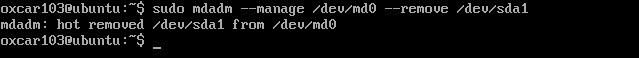
\includegraphics[width=15cm]{Ejercicio_2c.jpg}
			\caption{Extracción del dispositivo.}
			\label{fig:delete}
		\end{figure}
		
		Y ésta sería la salida que se nos muestra con el monitor dado, como podemos ver, el dispositivo
		ya no aparece:
		
		\begin{figure}[H]
			\centering
			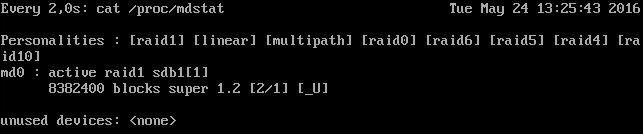
\includegraphics[width=15cm]{Ejercicio_2d.jpg}
			\caption{Estado de la máquina tras extraer el disco.}
			\label{fig:d_status}	
		\end{figure}
		
		Seguidamente, volvemos a añadirlo con el comando \verb|mdadm –-manage /dev/md0 –-add /dev/sda|:
		
		\begin{figure}[H]
			\centering
			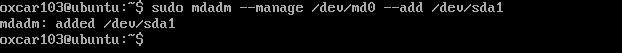
\includegraphics[width=15cm]{Ejercicio_2e.jpg}
			\caption{Recuperación del RAID dañado.}
			\label{fig:repair}	
		\end{figure}
		
		Al utilizar el monitor, volvemos a ver el dispositivo que habíamos quitado y vemos que se está
		reconstruyendo el RAID:
		
		\begin{figure}[H]
			\centering
			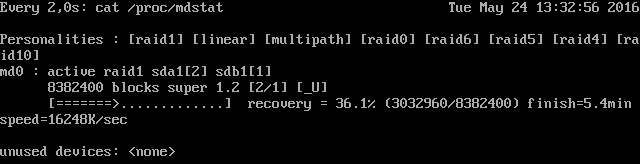
\includegraphics[width=15cm]{Ejercicio_2f.jpg}
			\caption{Progreso de la reconstrucción del RAID.}
			\label{fig:r_status}	
		\end{figure}
		
		Finalmente, queda así:
		
		\begin{figure}[H]
			\centering
			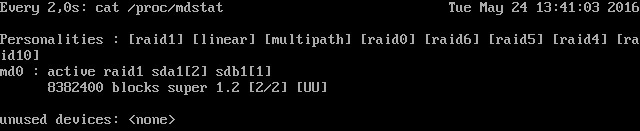
\includegraphics[width=15cm]{Ejercicio_2g.jpg}
			\caption{Estado final del RAID.}
			\label{fig:f_status}	
		\end{figure}
		
	\subsection{Programación de tareas con \textit{cron}}
		\item ¿Qué archivo ha de modificar para programar una tarea? Escriba la línea necesaria para
		ejecutar una vez al día una copia del directorio \verb|~|/codigo a \verb|~|/seguridad/
		\$fecha donde \$fecha es la fecha actual (puede usar el comando \textit{date}).
		
		En principio, el demonio \textit{cron}\cite{man_cron} ejecuta los comandos siguiendo las
		instrucciones dadas por el archivo \textit{crontab}\cite{man_crontab} y dispone además de una
		serie de repositorios con el fin de almacenar scripts con una periodicidad particular:
		\begin{itemize}
			\item \verb|/etc/cron.d| para ejecuciones de cualquier periodicidad.
			\item \verb|/etc/cron.hourly| para ejecuciones cada hora.
			\item \verb|/etc/cron.dialy| para ejecuciones cada día.
			\item \verb|/etc/cron.weekly| para ejecuciones cada semana.
			\item \verb|/etc/cron.monthly| para ejecuciones cada mes.
		\end{itemize}
		
		Para la tarea que nos piden realizar, creamos el siguiente script\footnote{He incluido el script
		directamente y se tienen ciertos errores en la visualización del $\%$.}:
		
		\lstinputlisting{./script.sh}
		
		Y como queremos programar que la tarea se repita de forma diaria, la incluiremos en el directorio
		\verb|/etc/cron.dialy/| anteriormente mencionado.
		
	\subsection{Analizando qué ocurre en el \textit{kernel} con \textit{dmesg}}
		\item Pruebe a ejecutar el comando, conectar un dispositivo USB y vuelva a ejecutar el
		comando. Copie y pegue la salida del comando (considere usar \verb+dmesg | tail+). Comente
		qué observa en la información mostrada.
		
		El comando \textit{dmesg}\cite{man_dmesg} nos muestra la información del \textit{kernel ring
		buffer} por defecto aunque dispone de algunos otros parámetros para darle formato y/o color a
		dicha salida o limpiar dicho buffer.
		
		Como resulta que tenía conectados tanto el móvil como el pendrive al portátil, he podido ver las
		líneas que hacen mención a cuándo lo conecté por primera vez, cuándo los desconecté y cuándo los
		he vuelto a conectar:
		
		\begin{figure}[H]
			\centering
			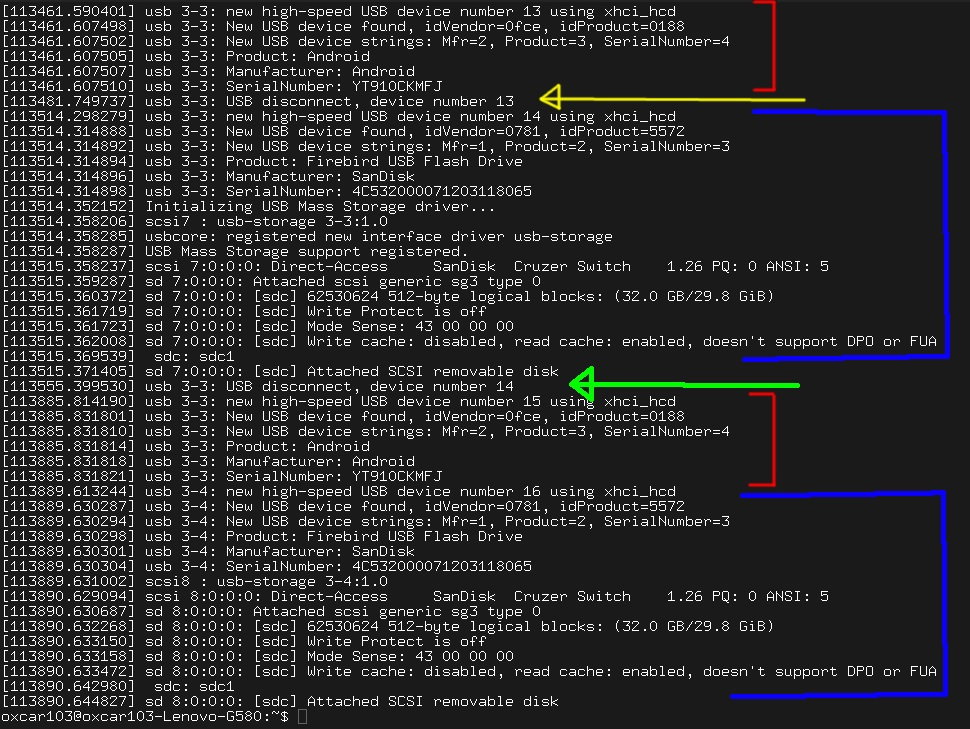
\includegraphics[width=15cm]{Ejercicio_4.jpg}
			\caption{Ejecución del comando \textit{dmesg}.}
			\label{fig:dmesg}	
		\end{figure}
		
		\begin{itemize}
			\item En rojo, las conexiones del móvil, nos muestra algunos datos del mismo como su número
			de serie.
			
			\item En amarillo, las desconexiones del móvil\footnote{De hecho, la desconexión que aparece,
			no es cosa mía, al parecer, el cable está un poco roto y se desconecta antes de que lo
			desenchufe, ya que lo desenchufé junto con el pendrive.}.
			
			\item En azul, las conexiones del pendrive, también nos muestra el número de serie, y además,
			se ve cómo se abre la carpeta cuando lo conectamos.
			
			\item En verde, las desconexiones del pendrive\footnote{Nótese, que no hay diferencia con
			las del móvil.}.
		\end{itemize}
		
	\subsection{Monitor General \textit{gnome-system-monitor}}
	\section{Monitorizando Windows: \textit{perfmon}}
		\item Ejecute el monitor de $"$System Performance$"$ y muestre el resultado. Incluya capturas
		de pantalla comentando la información que aparece.
		
		\item Cree un recopilador de datos definido por el usuario (modo avanzado) que incluya tanto
		el contador de rendimiento como los datos de seguimiento:
		\begin{itemize}
			\item Todos los referentes al procesador, al proceso y al servicio web.
			\item Intervalo de muestra 15 segundos
			\item Almacene el resultado en el directorio Escritorio$\backslash$logs
		\end{itemize}
		Incluya las capturas de pantalla de cada paso.
		
	\section{Monitorizando el hardware}
		\item instale alguno de los monitores comentados arriba en su máquina y pruebe a ejecutarlos
		(tenga en cuenta que si lo hace en la máquina virtual, los resultados pueden no ser
		realistas). Alternativamente, busque otros monitores para hardware comerciales o de código
		abierto para Windows y Linux.
		
	\section{Otros monitores del sistema}
	\subsection{Munin}
		\item Visite la web del proyecto y acceda a la demo que proporcionan
		(\url{http://demo.munin-monitoring.org/}) donde se muestra cómo monitorizan un servidor.
		Monitorice varios parámetros y haga capturas de pantalla de lo que está mostrando comentando
		qué observa.
	\subsection{Nagios}
		\item \textbf{Opcional:} Instale Nagios en su sistema (el que prefiera) documentando el
		proceso y muestre el resultado de la monitorización de su sistema comentando qué aparece.
		
	\subsection{Ganglia}
		\item \textbf{Opcional:} Haga lo mismo que con Munin.
		
	\subsection{Zabbix}
		\item \textbf{Opcional:} Prueba a instalar este monitor en alguno de sus tres sistemas.
		Realice capturas de pantalla del proceso de instalación y comente capturas de pantalla
		del programa en ejecución.
		
	\subsection{Cacti}
		\item \textbf{Opcional:} Pruebe a instalar este monitor en alguno de sus tres sistemas.
		Realice capturas de pantalla del proceso de instalación y comente capturas de pantalla
		del programa en ejecución.
		
	\subsection{Awstat}
		\item \textbf{Opcional:} Instale el monitor y muestre y comente algunas capturas de pantalla.
		
	\subsection{Monitorizando un servicio (o ejecución de un programa)}
		\item Escriba un breve resumen sobre alguno de los artículos donde se muestra el uso de
		\textit{strace}, o busque otro programa similar y coméntelo.
		
	\section{Profiling}
	\subsection{Ejecución de programas}
	\subsubsection{\textit{Gproof} y \textit{valgrind}}
		\item \textbf{Opcional:} Desarrolle una página en C o C++ y analice su comportamiento usando
		\textit{valgrind}. Visite \url{http://www.cs.tut.fi/~jkorpela/forms/cgic.html} para ver un
		ejemplo sencillo de una página web generada por un programa escrito en C.
		
	\subsubsection{PHP}
		\item \textbf{Opcional:} Desarrolle un script en PHP y analice su ejecución con alguno (o
		los dos) \textit{profilers}.
		
	\subsubsection{Python}
		\item \textbf{Opcional:} Escriba un script en python y analice su comportamiento usando el
		\textit{profiler} presentado.
		
	\subsubsection{PowerShell}
		\item \textbf{Opcional:} Escriba un script en PowerShell y analice su comportamiento
		usando el \textit{profiler} presentado.
		
	\subsection{Bases de Datos}
	\subsubsection{MySQL}
		\item Acceda a la consola mysql (o a través de phpMyAdmin) y muestre el resultado de mostrar
		el $"$profile$"$ de una consulta (la creación de la BD y la consulta la puede hacer libremente).
		
		Para testear el uso de dicho \textit{profile}, probaremos a realizar una consulta sobre una
		consulta sin índices y posteriormente, le incorporaremos uno para ver si se produce una mejora
		en la eficiencia de la misma\footnote{Aunque los índices suelen agilizar las búsquedas si están
		hechos sobre los campos adecuados, en algunas ocasiones como el hecho de incorporarlos en una
		tabla demasiado pequeña, un índice puede incluso empeorar el resultado. Sin embargo, en este
		experimento no se ha dado dicho caso.}.
		
		Sobre la base de datos por defecto \textit{mysql}, he realizado la consulta:
		\begin{verbatim}
			select password from user where user.user in (select user from proxies\_priv where
			with\_grant$>$0 \&\& host like '\%oxcar103\%');
		\end{verbatim}
		
		Después, he creado un índice sobre la tabla \textit{proxies\_priv} para agilizar la consulta.
		
		Y podemos ver el resultado en la siguiente captura del proceso\footnote{He emborronado la salida
		de la consulta porque no es de interés para la práctica y son contraseñas, aunque cifradas.}:
		
		\begin{figure}[H]
			\centering
			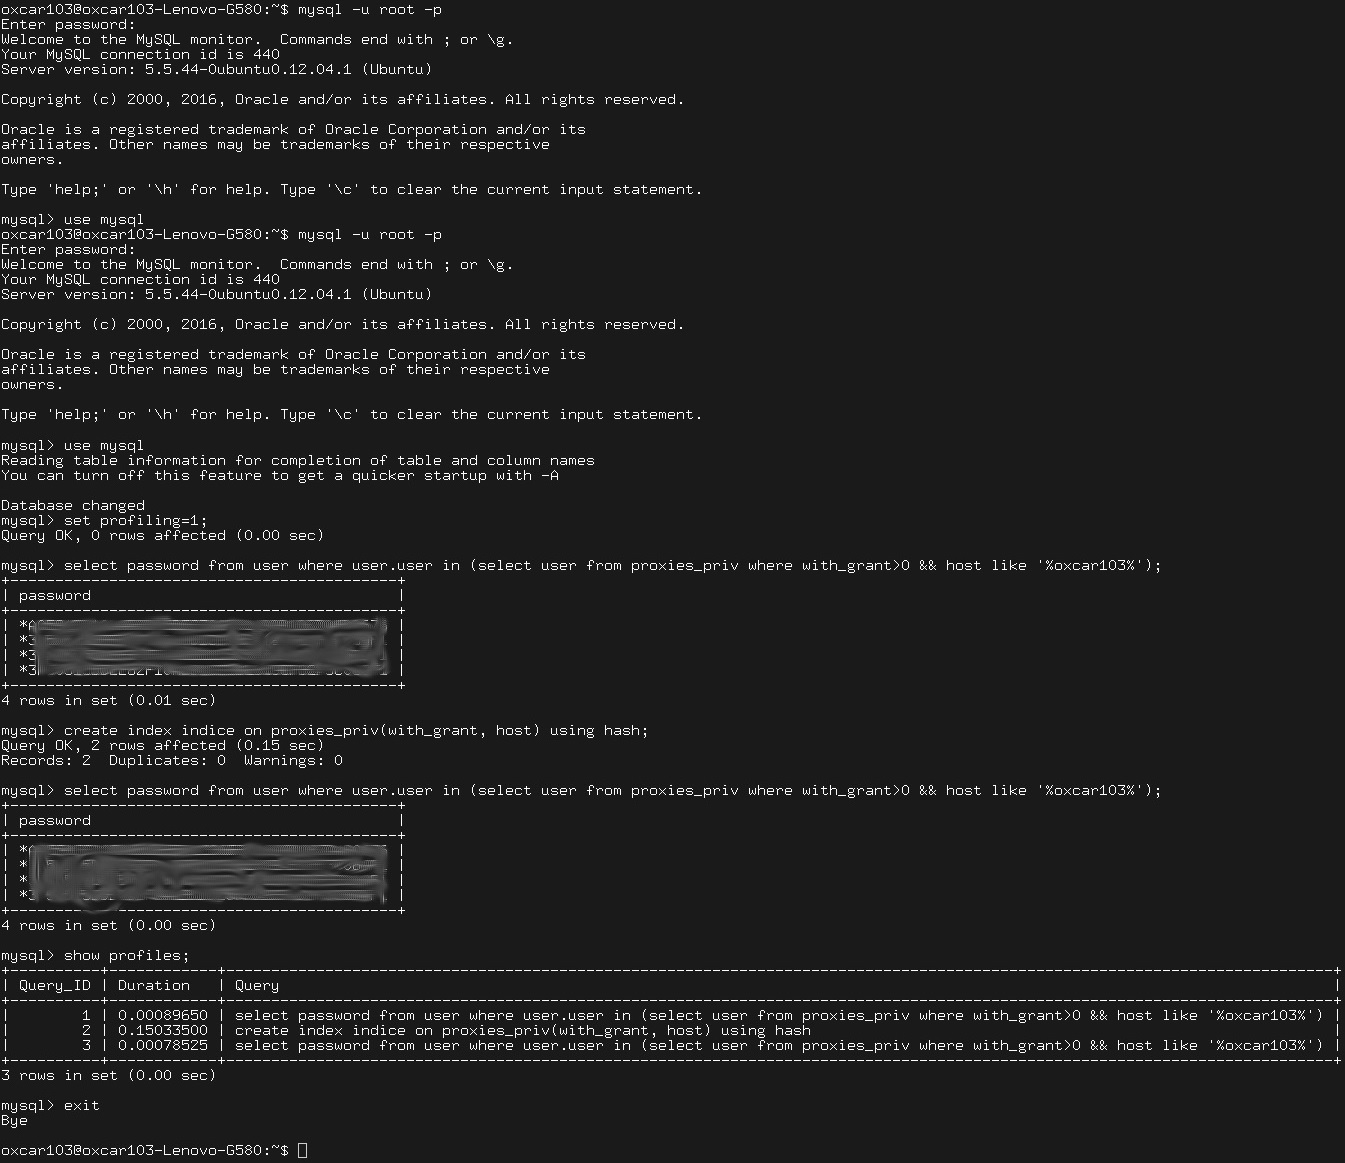
\includegraphics[width=15cm]{Ejercicio_19.jpg}
			\caption{Experimento con el \textit{profile} de \textit{mysql}.}
			\label{fig:profile}	
		\end{figure}
		
	\subsubsection{MongoDB}
		\item \textbf{Opcional:} Al igual que ha realizado el $"$profiling$"$ con MySQL, realice lo
		mismo con MongoDB y compare los resultados (use la misma información y la misma consulta, hay
		traductores de consultas SQL a Mongo).
		
\end{enumerate}

\newpage
\section{Referencias}
\begin{thebibliography}{10}
\expandafter\ifx\csname url\endcsname\relax
  \def\url#1{\texttt{#1}}\fi
\expandafter\ifx\csname urlprefix\endcsname\relax\def\urlprefix{URL }\fi
\expandafter\ifx\csname href\endcsname\relax
  \def\href#1#2{#2} \def\path#1{#1}\fi

\bibitem{man_yum}
Ubuntu manuals\\
yum(8) - Linux man page\\
\url{http://manpages.ubuntu.com/manpages/xenial/en/man8/yum.8.html}

\bibitem{man_yum.conf}
Ubuntu manuals\\
yum.conf(5) - Linux man page\\
  \url{http://manpages.ubuntu.com/manpages/xenial/en/man5/yum.conf.5.html}

\bibitem{CentOS_web}
CentOS.org\\
10. Using yum with a Proxy Server\\
  \url{https://www.centos.org/docs/5/html/yum/sn-yum-proxy-server.html}

\bibitem{foro_Fedora}
Fedoraforum.org\\
A fedora linux support community\\
  \url{http://forums.fedoraforum.org/showthread.php?t=742}

\bibitem{man_yum-config-manager}
Ubuntu manuals\\
yum-config-manager(1) - Linux man page\\
  \url{http://manpages.ubuntu.com/manpages/xenial/en/man1/yum-config-manager.1.html}

\bibitem{man_apt-cache}
Ubuntu manuals\\
apt-cache(8) - Linux man page\\
  \url{http://manpages.ubuntu.com/manpages/xenial/en/man8/apt-cache.8.html}

\bibitem{man_apt-get}
Ubuntu manuals\\
apt-get(8) - Linux man page\\
  \url{http://manpages.ubuntu.com/manpages/xenial/en/man8/apt-get.8.html}

\bibitem{man_apt.conf}
Ubuntu manuals\\
apt.conf(5) - Linux man page\\
  \url{http://manpages.ubuntu.com/manpages/wily/en/man5/apt.conf.5.html}

\bibitem{man_add-apt-repository}
Ubuntu manuals\\
add-apt-repository\\
  \url{http://manpages.ubuntu.com/manpages/natty/man1/add-apt-repository.1.html}

\bibitem{man_apt}
Ubuntu manuals\\
apt(8) - Linux man page\\
  \url{http://manpages.ubuntu.com/manpages/xenial/en/man8/apt.8.html}

\bibitem{oS_packman}
The openSUSE wiki\\
Package Management\\
  \url{https://en.opensuse.org/Package_management}

\bibitem{oS_YaST}
The openSUSE wiki\\
YaST Software Management\\
  \url{https://en.opensuse.org/Portal:YaST}

\bibitem{oS_zypper}
The openSUSE wiki\\
Zypper\\
  \url{https://en.opensuse.org/Portal:Zypper}

\bibitem{oS_YaST_GitHub}
GitHub - How people build software\\
YaST\\
  \url{https://github.com/yast}

\bibitem{oS_zypper_GitHub}
GitHub - How people build software\\
Zypper - Según su propia descripción: "World's most powerful command line package manager"\\
  \url{https://github.com/openSUSE/zypper}

\bibitem{Telnet}
Telnet. Wikipedia, the free encyclopedia.\\
  \url{https://en.wikipedia.org/wiki/Telnet}

\bibitem{SSH}
Secure Shell. Wikipedia, the free encyclopedia.\\
  \url{https://en.wikipedia.org/wiki/Secure_Shell}

\bibitem{man_SSH}
Ubuntu manuals\\
ssh(1) - Linux man page\\
  \url{http://manpages.ubuntu.com/manpages/xenial/en/man1/ssh.1.html}

\bibitem{SSH_StackOverFlow}
StackOverFlow. \\
How to SSH to a VirtualBox guest externally through a host? \\
  \url{http://stackoverflow.com/questions/5906441/how-to-ssh-to-a-virtualbox-guest-externally-through-a-host}

\bibitem{man_ssh-keygen}
Ubuntu manuals\\
ssh-keygen(1) - Linux man page\\
  \url{http://manpages.ubuntu.com/manpages/xenial/en/man1/ssh-keygen.1.html}

\bibitem{man_ssh-copy-id}
Ubuntu manuals\\
ssh-copy-id(1) - Linux man page\\
  \url{http://manpages.ubuntu.com/manpages/xenial/en/man1/ssh-copy-id.1.html}

\bibitem{man_apropos}
Ubuntu manuals\\
apropos(1) - Linux man page\\
  \url{http://manpages.ubuntu.com/manpages/xenial/en/man1/apropos.1.html}

\bibitem{man_service}
Ubuntu manuals\\
service(8) - Linux man page\\
  \url{http://manpages.ubuntu.com/manpages/xenial/en/man8/service.8.html}

\bibitem{man_systemctl}
Ubuntu manuals\\
systemctl(1) - Linux man page\\
  \url{http://manpages.ubuntu.com/manpages/xenial/en/man1/systemctl.1.html}

\bibitem{man_fail2ban}
Ubuntu manuals\\
fail2ban(1) - Linux man page\\
  \url{http://manpages.ubuntu.com/manpages/xenial/en/man1/fail2ban.1.html}

\bibitem{man_jail.conf}
Ubuntu manuals\\
jail.conf(5) - Linux man page\\
  \url{http://manpages.ubuntu.com/manpages/xenial/en/man1/jail.conf.10.html}

\bibitem{man_sshd_config}
Ubuntu manuals\\
sshd\_config(5) - Linux man page\\
  \url{http://manpages.ubuntu.com/manpages/xenial/en/man5/sshd_config.5.html}

\bibitem{man_nano}
Ubuntu manuals\\
nano(1) - Linux man page\\
  \url{http://manpages.ubuntu.com/manpages/xenial/en/man1/nano.1.html}

\bibitem{TWG}
GitHub - How people build software\\
Análisis comparativo de Tomcat, WildFly y GlassFish\\
  \url{https://github.com/oxcar103/Trabajo-ISE}

\bibitem{TC_official}
\textbf{Apache Tomcat}\\
  \url{http://tomcat.apache.org/}

\bibitem{WF_official}
\textbf{JBossDeveloper}\\
  \url{http://wildfly.org/}\\
  \url{http://jbossas.jboss.org/}\footnote{Antiguo enlace a la página oficial, al parecer, esta página
  ha dejado de estar disponible, luego éste ya no está operativo pero me parece que tiene cierto
  interés histórico.}\\

\bibitem{GF_official}
\textbf{GlassFish}\\
  \url{https://glassfish.java.net/}

\bibitem{GF_install}
\textbf{\textit{Java EE 7 with GlassFish 4 Application Server}}\\
David R. Heffelfinger\\
Ed. Packt Publishing (March 2014)\\
Sec. "1. Getting Started with GlassFish"\\
  \url{http://proquest.safaribooksonline.com/book/programming/java/9781782176886}

\bibitem{TC_install}
\textbf{\textit{Apache Tomcat 7 Essentials}}\\
Tanuj Khare\\
Ed. Packt Publishing (March 2012)\\
Sec. "1. Installation of Tomcat7"\\
  \url{http://proquest.safaribooksonline.com/book/operating-systems-and-server-administration/apache/9781849516624}

\bibitem{TC_download}
\textbf{Apache Tomcat}\\
  \url{http://tomcat.apache.org/download-70.cgi}

\bibitem{TC_StackOverFlow}
\textbf{Stack Overflow}
  \url{http://stackoverflow.com/questions/4756039/how-to-change-the-port-of-tomcat-from-8080-to-80}

\bibitem{WF_install}
\textbf{\textit{WildFly: New Features}}\\
Filippe Costa Spolti\\
Ed. Packt Publishing (May 2014)\\
Sec. "1. Starting with WildFly"\\
  \url{http://proquest.safaribooksonline.com/9781783285891?uicode=goliat} 

\bibitem{WF_download}
\textbf{JBossDeveloper}\\
  \url{http://wildfly.org/downloads/}

\bibitem{WF_solution}
\textbf{Dmitriy Sukharev. IT Blog}\\
  \url{http://sukharevd.net/wildfly-8-installation.html}
  \url{https://gist.github.com/sukharevd/6087988}

\bibitem{man_diff}
Ubuntu manuals\\
diff(1) - Linux man page\\
  \url{http://manpages.ubuntu.com/manpages/xenial/en/man1/diff.1posix.html}

\bibitem{man_patch}
Ubuntu manuals\\
patch(1) - Linux man page\\
  \url{http://manpages.ubuntu.com/manpages/xenial/en/man1/patch.1.html}

\bibitem{webmin}
Webmin.com\\
Using the Webmin APT repository\\
  \url{http://webmin.com/deb.html}

\bibitem{man_php}
Ubuntu manuals\\
php(1) - Linux man page\\
  \url{http://manpages.ubuntu.com/manpages/precise/en/man1/php.1.html}

\bibitem{ispconfig}
ispconfig.org\\
Online demo\\
  \url{http://www.ispconfig.org/ispconfig/online-demo/}

\bibitem{man_find}
Ubuntu manuals\\
find(1) - Linux man page\\
  \url{http://manpages.ubuntu.com/manpages/xenial/en/man1/find.1.html}

\bibitem{man_grep}
Ubuntu manuals\\
grep(1) - Linux man page\\
  \url{http://manpages.ubuntu.com/manpages/xenial/en/man1/grep.1posix.html}

\bibitem{man_sed}
Ubuntu manuals\\
sed(1) - Linux man page\\
  \url{http://manpages.ubuntu.com/manpages/xenial/en/man1/sed.1posix.html}

\bibitem{man_awk}
Ubuntu manuals\\
awk(1) - Linux man page\\
  \url{http://manpages.ubuntu.com/manpages/xenial/en/man1/awk.1plan9.html}

\end{thebibliography}


\end{document}